\section{Ejercicio 5 - Lote para Round Robin}

Se diseñó un lote con 3 tareas de tipo {\tt TaskCPU} de 50 ciclos y 2 de tipo {\tt TaskConsola} con 5 llamadas bloqueantes de 3 ciclos de duración cada una.  Las Figuras \ref{fig-rrq2}, \ref{fig-rrq10} y \ref{fig-rrq50} muestran los resultados de la simulación de este lote con el scheduler Round Robin implementado, con quantum de 2, 10 y 50 ciclos respectivamente.

\begin{figure}[!htb]
\begin{center}
  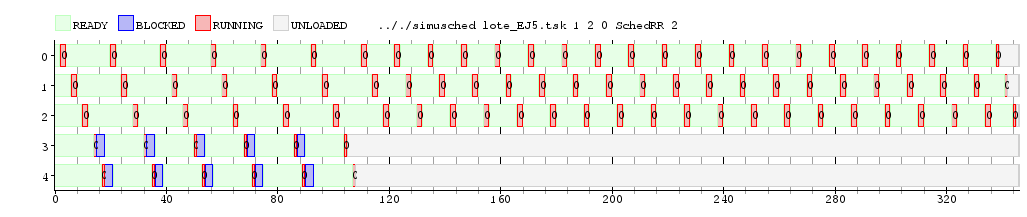
\includegraphics[scale=0.45]{imagenes/ej5-q2.png}
\end{center}
\caption{Simulación para SchedRR, 1 núcleo, quantum 2 y 2 ciclos de cs}\label{fig-rrq2}
\end{figure}

\begin{figure}[!htb]
\begin{center}
  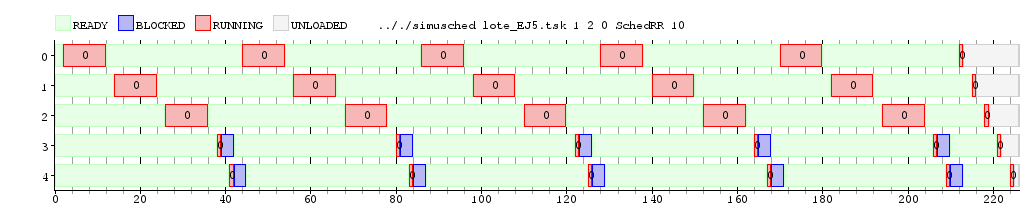
\includegraphics[scale=0.45]{imagenes/ej5-q10.png}
\end{center}
\caption{Simulación para SchedRR, 1 núcleo, quantum 10 y 2 ciclos de cs}\label{fig-rrq10}
\end{figure}

\begin{figure}[!htb]
\begin{center}
  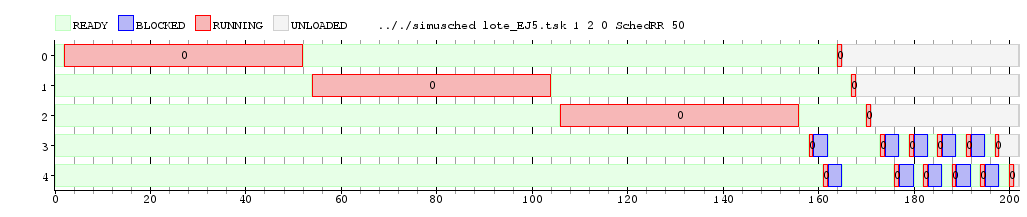
\includegraphics[scale=0.45]{imagenes/ej5-q50.png}
\end{center}
\caption{Simulación para SchedRR, 1 núcleo, quantum 50 y 2 ciclos de cs}\label{fig-rrq50}
\end{figure}

Para cada caso simulado, se calculó la latencia, el waiting-time y el tiempo total de ejecución para las 5 tareas del lote. El Cuadro \ref{tab-datos} muestra los datos obtenidos y el Cuadro \ref{tab-promedios} muestra los promedios de las 5 tareas para cada quantum.

\begin{table}[!htb]
\begin{center}
\begin{tabular}{| l | l | l | l | l |}
\hline
Task & Quantum & Latecia & Waiting-time & Total ejecución\\
\hline
0 	& 2 & 2 & 288 & 339\\
	& 10& 2 & 162 & 213\\
	& 50& 2 & 114 & 165\\
\hline
1	& 2 & 6 & 291 & 342\\
	& 10& 14& 165 & 216\\
	& 50& 54& 117 & 168\\
\hline
2	& 2 & 10 & 294 & 345\\
	& 10& 26 & 168 & 219\\
	& 50& 106& 120 & 171\\
\hline
3	& 2 & 14 & 84 & 105\\
	& 10& 38 & 201& 222\\
	& 50& 158& 177& 198\\
\hline
4	& 2 & 17 & 87 & 108\\
	& 10& 41 & 204&	225\\
	& 50& 161& 180& 201\\
\hline
\end{tabular}
\end{center}
\caption{Datos de simulación - SchedRR}\label{tab-datos}
\end{table}

%\vspace*{0.5cm}

Basándonos en los promedios calculados, el mejor caso de los simulados para latencia es el que utiliza quantum de 2 ciclos, lo cual puede explicarse dado que teniendo un quantum tan corto, todos los procesos entran en la ronda de ejecución rápidamente. Respecto a waiting-time, el mejor es el caso con quantum de 50 ciclos, y puede deberse a que al tener más ciclos por quantum el tiempo de cambio de contexto tiene menor impacto en el tiempo total de espera.  Por último, el mejor tiempo total de ejecución lo tiene también el caso con 50 ciclos de quantum, y estimamos que también tiene que ver el impacto del tiempo invertido en realizar cada cambio de contexto.

Podríamos concluir entonces que, dependiendo de las tareas que se estén ejecutando, si no es primordial que el tiempo de respuesta sea mínimo, utilizar un quantum de 50  ciclos parecería aprovechar de mejor manera los recursos del procesador. Sin embargo, si es prioritario obtener una respuesta sin importar que esto provoque  que las tareas demoren mucho tiempo en finalizarse, convendría utilizar el quantum con 2 ciclos.